\documentclass[12pt,a4paper]{article}
\usepackage[T1]{fontenc}
\usepackage[spanish,es-nodecimaldot]{babel}
\usepackage{tgtermes}
\usepackage{newtxmath}
\usepackage{amsmath}
\usepackage{textcomp}
\usepackage{graphicx}
\usepackage{geometry}
\usepackage{xcolor}
\usepackage{setspace}
\usepackage{titlesec}
\usepackage{tocloft}
\usepackage{fancyhdr}
\usepackage{enumitem}
\usepackage{hyperref}

\geometry{margin=2.5cm}

\definecolor{AzulPrincipal}{HTML}{0B2D4D}
\definecolor{AzulSecundario}{HTML}{1F5F8B}
\definecolor{OroAcento}{HTML}{C9A227}
\definecolor{GrisTexto}{HTML}{444444}

\hypersetup{
    colorlinks=true,
    linkcolor=black,
    urlcolor=black,
    citecolor=black,
    pdftitle={Plantilla de Informe},
    pdfauthor={Tu Nombre}
}

\setlength{\parindent}{1.25cm}
\setlength{\parskip}{0.25em}
\onehalfspacing

\setlist[itemize]{leftmargin=2.8em, labelsep=0.8em, topsep=0.35em, itemsep=0.2em}
\setlist[enumerate]{leftmargin=1.7em, topsep=0.35em, itemsep=0.2em}

\titleformat{\section}[hang]{\fontsize{18pt}{22pt}\selectfont\normalfont\color{black}}{\thesection.}{0.8em}{}
\titleformat{\subsection}[hang]{\fontsize{14pt}{17pt}\selectfont\normalfont\color{black}}{\thesubsection}{0.8em}{}

\renewcommand{\cftsecfont}{\normalfont}
\renewcommand{\cftsecpagefont}{\normalfont}
\renewcommand{\cftsubsecfont}{\normalfont}
\renewcommand{\cftsubsecpagefont}{\normalfont}
\renewcommand{\cftsecleader}{\cftdotfill{\cftdotsep}}
\renewcommand{\cftsubsecleader}{\cftdotfill{\cftdotsep}}
\renewcommand{\contentsname}{Índice}
\renewcommand{\cfttoctitlefont}{\hfill\normalfont\fontsize{18pt}{22pt}\selectfont}
\renewcommand{\cftaftertoctitle}{\hfill}

\titlespacing*{\section}{0pt}{1.1em}{0.55em}
\titlespacing*{\subsection}{0pt}{0.9em}{0.35em}

\setlength{\headheight}{30pt}

\pagestyle{fancy}
\fancyhf{}
\lhead{\small\textcolor{black!65}{\Laboratorio: \Tema}}
\rhead{}
\cfoot{\small\textcolor{black}{\thepage}}
\renewcommand{\headrulewidth}{0.4pt}
\renewcommand{\headrule}{\hbox to\headwidth{\color{black!65}\leaders\hrule height \headrulewidth\hfill}}
\renewcommand{\footrulewidth}{0pt}

\providecommand{\Universidad}{UNIVERSIDAD NACIONAL DE INGENIERÍA}
\providecommand{\Facultad}{FACULTAD DE CIENCIAS}
\providecommand{\Escuela}{ESCUELA DE FÍSICA}
\providecommand{\Curso}{CIRCUITOS ELÉCTRICOS ANALÓGICOS}
\providecommand{\Seccion}{SECCIÓN A}
\providecommand{\NumeroLaboratorio}{X}
\providecommand{\Laboratorio}{LABORATORIO N\textdegree{} \NumeroLaboratorio}
\providecommand{\Tema}{TÍTULO DE LA PRÁCTICA}
\providecommand{\RutaLogo}{logo.PNG}
\providecommand{\IntegrantesBloque}{%
\begin{enumerate}[leftmargin=1.8em,label=\arabic*.]
    \item Integrante 1 -- código
    \item Integrante 2 -- código
\end{enumerate}}
\providecommand{\FechaRealizacion}{Fecha de realización: dd de mes de aaaa - hh:mm}
\providecommand{\Ciudad}{LIMA - PERU}

\newcommand{\ConfigurarInforme}[3]{%
    \renewcommand{\NumeroLaboratorio}{#1}%
    \renewcommand{\Tema}{#2}%
    \renewcommand{\FechaRealizacion}{#3}%
}

\newcommand{\ConfigurarIntegrantes}[1]{%
    \renewcommand{\IntegrantesBloque}{#1}%
}

\providecommand{\tituloSeccion}[1]{\section{#1}}

\providecommand{\makeInformePortada}{%
\begin{titlepage}
    \thispagestyle{empty}
    \vspace*{0.65cm}
    \begin{center}
        {\Large\bfseries\color{OroAcento} \Universidad}\par
        \vspace{0.45cm}
        {\Large\bfseries\color{AzulPrincipal} \Facultad}\par
        \vspace{0.25cm}
        {\Large\bfseries\color{AzulPrincipal} \Escuela}\par
    \end{center}

    \vspace{0.1cm}
    \begin{center}
        \includegraphics[width=0.4\textwidth]{\RutaLogo}%
    \end{center}

    \vspace{0.01cm}
    \begin{center}
        {\Large\bfseries\color{AzulPrincipal} \Curso}\par
        \vspace{0.35cm}
        {\Large\bfseries\color{red} \Seccion}\par
    \end{center}

    \vspace{0.1cm}
    \begin{center}
        {\large\bfseries \Laboratorio: \Tema}\par
    \end{center}

    \vspace{0.55cm}
    \noindent{\large\textbf{INTEGRANTES DE LA MESA:} 2}\par
    \vspace{0.35cm}
    \begingroup
    \leftskip=1.15cm
    \rightskip=1.15cm
    \parindent=0pt
    \IntegrantesBloque
    \endgroup

    \vspace{0.55cm}
    \begin{center}
        {\FechaRealizacion}\par
    \end{center}

    \vfill

    \begin{center}
        {\large\bfseries \Ciudad}
    \end{center}
\end{titlepage}
}
\usepackage{tikz}
\renewcommand{\RutaLogo}{../../PLANTILLA/logo.PNG}
\graphicspath{{Imagenes/}}
\ConfigurarInforme{1}{MEDICIONES DC}{Fecha de realización del Laboratorio N\textdegree{}1: Jueves 26 de Marzo del 2026 - 08:00 am}

% Inicio del informe
\begin{document}
\makeInformePortada
\setcounter{page}{1}
\tableofcontents
\newpage

% Contenido del informe
\tituloSeccion{Objetivos}
\subsection{Objetivo general}
    \begin{itemize}
        \item Realizar mediciones eléctricas básicas basadas en circuitos resistivos, utilizando un multímetro digital.
    \end{itemize}
\subsection{Objetivos específicos}
    \begin{itemize}
        \item Obtener valores de resistencias eléctricas utilizando la tabla del código de colores y un multímetro digital.
        \item Analizar el comportamiento de los circuitos divisores de voltaje y de corriente.
        \item Determinar la influencia de la impedancia interna del multímetro en mediciones de voltaje.
    \end{itemize}

\tituloSeccion{Fundamento Teórico}

\subsection{Resistor Eléctrico}
Un resistor es un componente muy usado en circuitos electrónicos, el cual posee un valor de resistencia $R$ especificado y nos sirve para regular los valores de corriente y voltaje según se requiera. En la práctica el valor de una resistencia varía en un cierto porcentaje según se especifique en su fabricación. En circuitos se pueden emplear resistores de valor fijo o variable (Fig. \ref{Resistoresvariables}).

\begin{figure}[H]
    \centering
    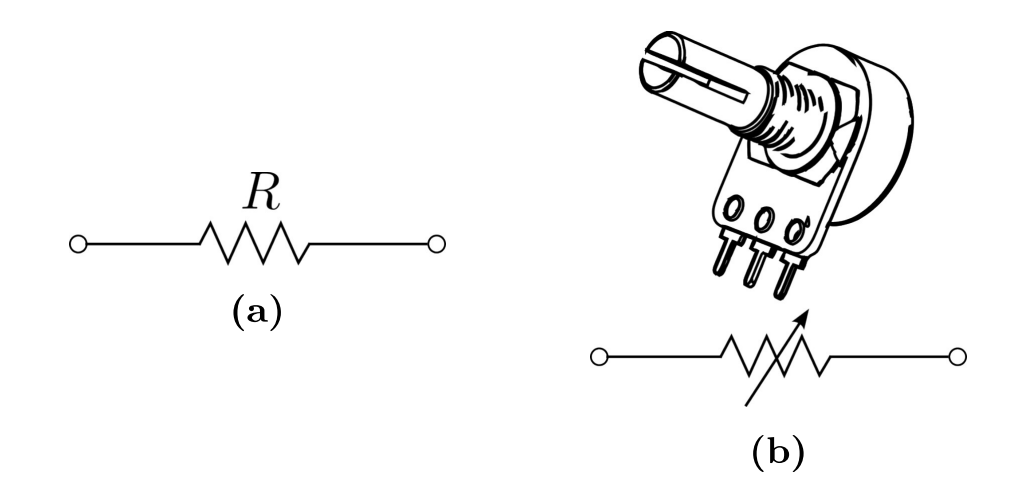
\includegraphics[width=0.6\linewidth]{Imagen1.PNG}
    \caption{Resistores de valor fijo (a) y variable (b)}
    \label{Resistoresvariables}
\end{figure}

La resistencia variable es denominada potenciómetro con tres terminales y una perilla.
Cuando se usan únicamente los terminales en los extremos se tiene el comportamiento de un resistor con un valor fijo y máximo.
Cuando se usa uno de los extremos y el terminal del medio, se comporta como una resistor variable, donde su resistencia se modifica haciendo girar la perilla. Su rango de valores no puede exceder el valor fijo máximo. Un resistor variable de dos terminales es conocido también como \textbf{reostato}.

Los resistores de bandas coloridas son muy usados debido a su bajo coste y fácil manipulación. Pueden ser de 4, 5 o 6 bandas, donde el orden y el color de cada una nos indican un valor de resistencia específico de acuerdo al código de color universal del resistor (Fig. \ref{RCodColores}).

\newpage
Las primeras bandas de colores nos indica un número compuesto según el orden en que están.
La penúltima banda conocida como \textbf{multiplicador} nos indica la potencia de 10 que se multiplicará al valor obtenido en las bandas anteriores.
La última banda nos indica la \textbf{tolerancia} que es el porcentaje en el que varía el valor obtenido anteriormente. Esta banda suele estar más alejada de las otras y por lo general es dorada o plateada.

Por ejemplo si tenemos un resistor de 5 bandas de colores: rojo, verde, marrón, rojo, dorado; se tendrá una resistencia $R = (25,100 \pm 1,255) k\Omega$

\begin{figure}[H]
    \centering
    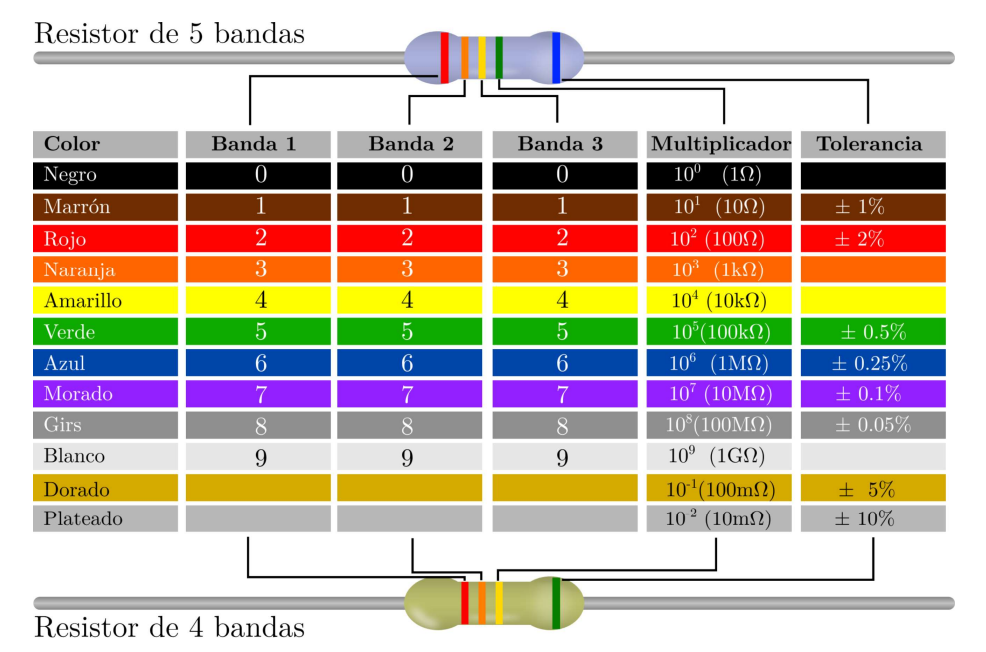
\includegraphics[width=0.8\linewidth]{Imagen2.PNG}
    \caption{Código de colores para resistores de 4 o 5 bandas}
    \label{RCodColores}
\end{figure}

Un conjunto de resistores en serie o en paralelo se comportan como un solo resistor con un valor de resistencia equivalente $R_{eq}$ específico. Para resistores en serie: 
\begin{equation}
    R_{eq} = R_1+R_2+...+R_n
    \label{eq:serie}
\end{equation}
y para resistores en paralelo:
\begin{equation}
    \frac{1}{R_{eq}} = \frac{1}{R_1} + \frac{1}{R_2} + \cdots + \frac{1}{R_n}
    \label{eq:paralelo}
\end{equation}

\begin{figure}[H]
    \centering
    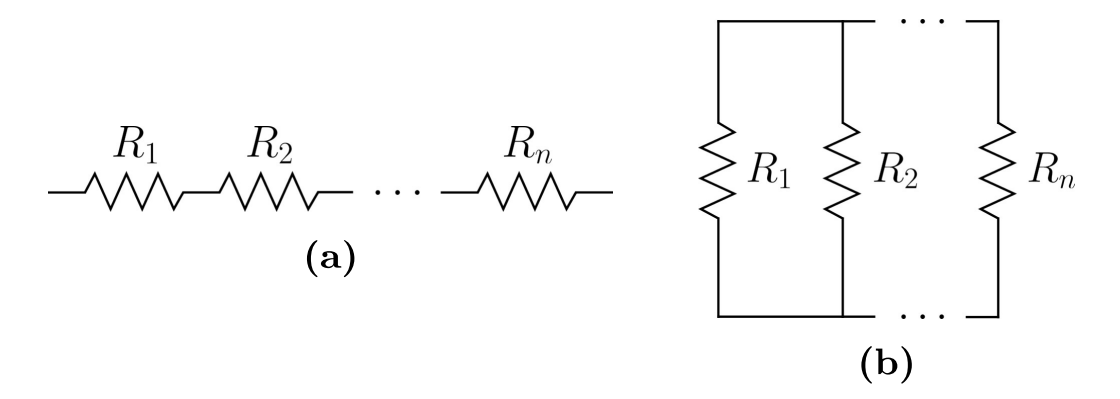
\includegraphics[width=0.8\linewidth]{Imagen3.PNG}
    \caption{Resistores en serie (a) y en paralelo (b)}
    \label{ResistoresSP}
\end{figure}

\subsection{Circuito divisor de voltaje}
Este circuito en serie se caracteriza porque la corriente es la misma (en una rama parcial del circuito), mientras que el voltaje $V$ se encuentra repartido o dividido proporcionalmente al valor de cada resistor (Fig. \ref{DivisorVoltaje}).

\begin{figure}[H]
    \centering
    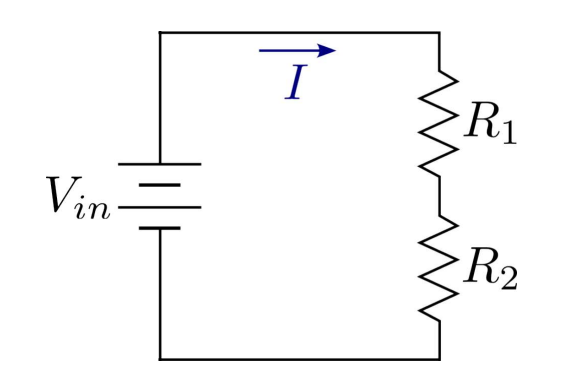
\includegraphics[width=0.5\linewidth]{Imagen4.PNG}
    \caption{Circuito divisor de voltaje}
    \label{DivisorVoltaje}
\end{figure}

Si por el circuito pasa una corriente $I$ entonces se tiene $V_{in} - IR_1 - IR_2=0$. Por la ley de Ohm, en el resistor $R_2$ se tiene que $V_2=IR_2$. Entonces:
\begin{equation}
    V_2=V_{in}\bigg(\frac{R_2}{R_1+R_2}\bigg)
    \label{eq:divisor-voltaje}
\end{equation}

Podemos generalizar esta ecuación para un circuito con $n$ resistores, de modo que en el voltaje en el resistor $i$ se obtenga como:
\begin{equation}
    V_i=V_{in}\bigg(\frac{R_i}{R_1+R_2+...+R_n}\bigg)
    \label{eq:divisor-voltaje-general}
\end{equation}

\subsection{Circuito divisor de corriente}
Este circuito en paralelo se caracteriza porque el voltaje $V$ es el mismo en cada rama del circuito, mientras que la corriente $I$ se encuentra repartida o dividida proporcionalmente al valor de cada resistor (Fig. \ref{DivisorCorriente}).

\begin{figure}[H]
    \centering
    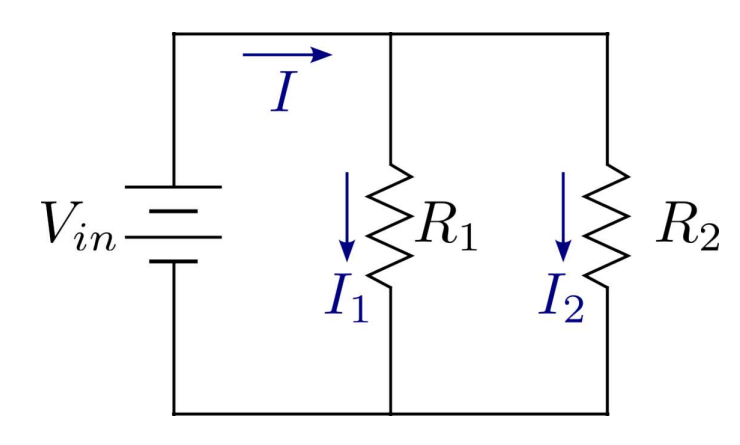
\includegraphics[width=0.5\linewidth]{Imagen5.PNG}
    \caption{Circuito divisor de corriente}
    \label{DivisorCorriente}
\end{figure}

La resistencia equivalente del circuito se calcula con la ecuación \ref{eq:paralelo}, de la cual obtenemos $R_{eq}=\frac{R_1R_2}{R_1+R_2}$, por lo tanto, $V_{in}-IR_{eq}=0$. Reemplazando esta ecuación en las ecuaciones $V_1-IR_1=0$ y $V_2-IR_2=0$, se obtiene:
\begin{equation}
    I_1=I\bigg(\frac{R_2}{R_1+R_2}\bigg) \quad\text{y}\quad I_2=I\bigg(\frac{R_1}{R_1+R_2}\bigg)
    \label{eq:divisor-corriente}
\end{equation}

Podemos generalizar esta ecuación para un circuito con $n$ resistores, de modo que en la corriente en el resistor $i$ se obtenga como:
\begin{equation}
    I_i=I\bigg(\frac{R_{eq}}{R_i}\bigg)
    \label{eq:divisor-corriente-general}
\end{equation}

\bigskip
\subsection{Impedancia del multímetro}
Un multímetro digital permite hacer mediciones de voltaje, corriente, resistencia, entre otros. Este cuenta con terminales de entrada donde unos cables con puntas realizan la medición; un selector rotativo para acceder a las diferentes funciones y rangos de medición; y una pantalla que muestra el número medido indicando también valores decimales, signo negativo si corresponde, la unidad de medida e incluso el tipo de corriente (DC o AC).

La impedancia interna del multímetro es una característica intrínseca que se presenta al realizar mediciones. Esta impedancia puede influir en los valores medidos porque interactúa con el circuito. La impedancia interna varía dependiendo de la función seleccionada, por ejemplo, al medir voltaje, la impedancia interna debería ser muy alta (idealmente infinita) de este modo la resistencia equivalente casi no se altera. Por otro lado, al medir corriente, la impedancia interna debería ser extremadamente baja (idealmente igual a cero). Es muy importante señalar que las medidas de voltaje se realizan en paralelo y las de corriente en serie.

\bigskip
\tituloSeccion{Materiales e indicaciones}

\begin{itemize}
    \item Fuente de voltaje DC: Fuente casera de voltaje continuo otorgado por la facultad, con salidas de voltaje predeterminadas como 1.5V, 5V y 15V, además de una perilla que regula la salida del voltaje y muestra en pantalla la cantidad exacta. Para su uso, se deben conectar los cables de salida a los terminales correspondientes del circuito, asegurándose de respetar la polaridad (positivo y negativo).
    \item Multímetro digital: Instrumento de medición, modelo PRASEK PREMIUM PR-61C, cuyos modos de operación son ohmímetro, voltímetro y amperímetro. Su número de dígitos es de 4 y presenta las siguientes escalas:
    \begin{enumerate}
        \item Resistencia: 600 $\Omega$, 6 $k\Omega$, 60 $k\Omega$, 600 $k\Omega$, 6 $M\Omega$ y 60 $M\Omega$.
        \item Voltaje: 60 mV, 600 mV, 6 V, 60 V, 600 V y 750 V.
        \item Corriente: 600 $\mu$A, 6000 $\mu$A, 60 mA, 600 mA, 6 A y 10 A.
        \item Impedancia de entrada: alrededor de 3000 $M\Omega$ en las escalas de 60 mV y 600 mV, y alrededor de 10 $M\Omega$ en las escalas de 6 V, 60 V, 600 V y 750 V.
    \end{enumerate}
    \newpage
    Para su uso, se deben conectar los cables de medición a los terminales correspondientes del multímetro, seleccionar la función deseada en el selector rotativo y realizar la medición en el circuito, asegurándose de respetar la polaridad y la configuración adecuada para cada tipo de medición.
    \item Protoboard: Es una placa de pruebas que permite realizar conexiones temporales sin necesidad de soldar. Para su uso, se deben insertar los componentes en las filas y columnas correspondientes, y realizar las conexiones utilizando cables de puente.
    \item Resistencias: Son componentes que limitan el flujo de corriente en un circuito. Para su uso, se deben identificar sus valores utilizando el código de colores o un multímetro, y conectarlas en el circuito según sea necesario.
    \item Potenciómetros: Son resistencias variables que permiten ajustar la resistencia manualmente. Para su uso, se deben conectar los terminales según el esquema del circuito y ajustar la perilla para obtener el valor de resistencia deseado.
\end{itemize}

\tituloSeccion{Procedimiento experimental}
\subsection{PASO 1: Medición de resistencias}
\begin{enumerate}
    \item Se escogieron 3 resistencias de cuatro bandas y 2 resistencias de 5 bandas y se registraron en la Tabla \ref{tab:medicion-resistencias} sus valores nominales y porcentajes de tolerancia según el código de colores, así como el valor real medido con el multímetro.
    \item Se armó el circuito indicado en la Figura \ref{CircuitoRedResistiva} en el protoboard, se escogieron 8 resistencias de 4 bandas, de valores diferentes pero de la misma magnitud. Se midió la resistencia equivalente entre A y B. También se encontró el error relativo entre el valor teórico y el valor medido. Los datos fueron anotados en las tablas \ref{tab:red-resistiva-resistencias} y \ref{tab:red-resistiva-resultados}.
    \begin{figure}[H]
        \centering
        \begin{minipage}{0.45\linewidth}
            \centering
            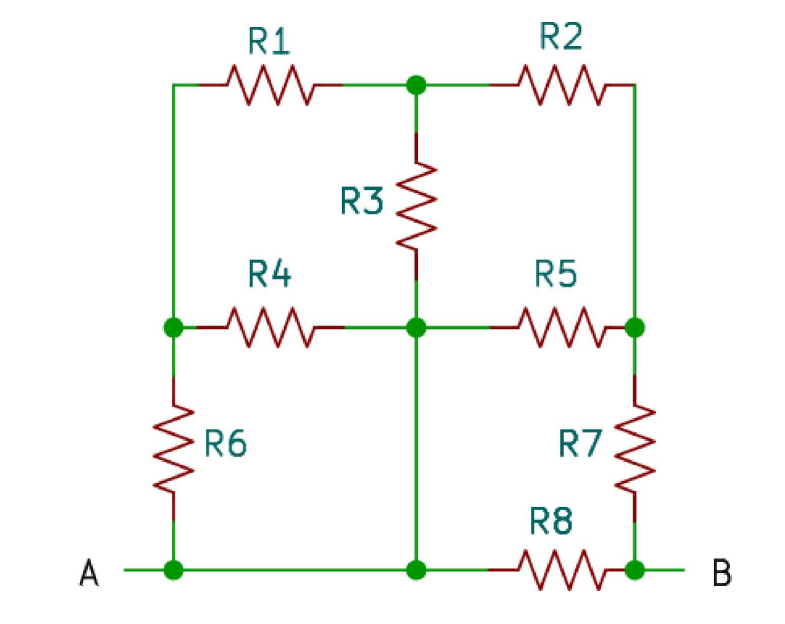
\includegraphics[width=\linewidth]{Imagen6.PNG}
            \caption{Circuito para medir la resistencia equivalente de una red resistiva}
            \label{CircuitoRedResistiva}
        \end{minipage}
        \hspace{0.02\linewidth}
        \begin{minipage}{0.45\linewidth}
            \centering
            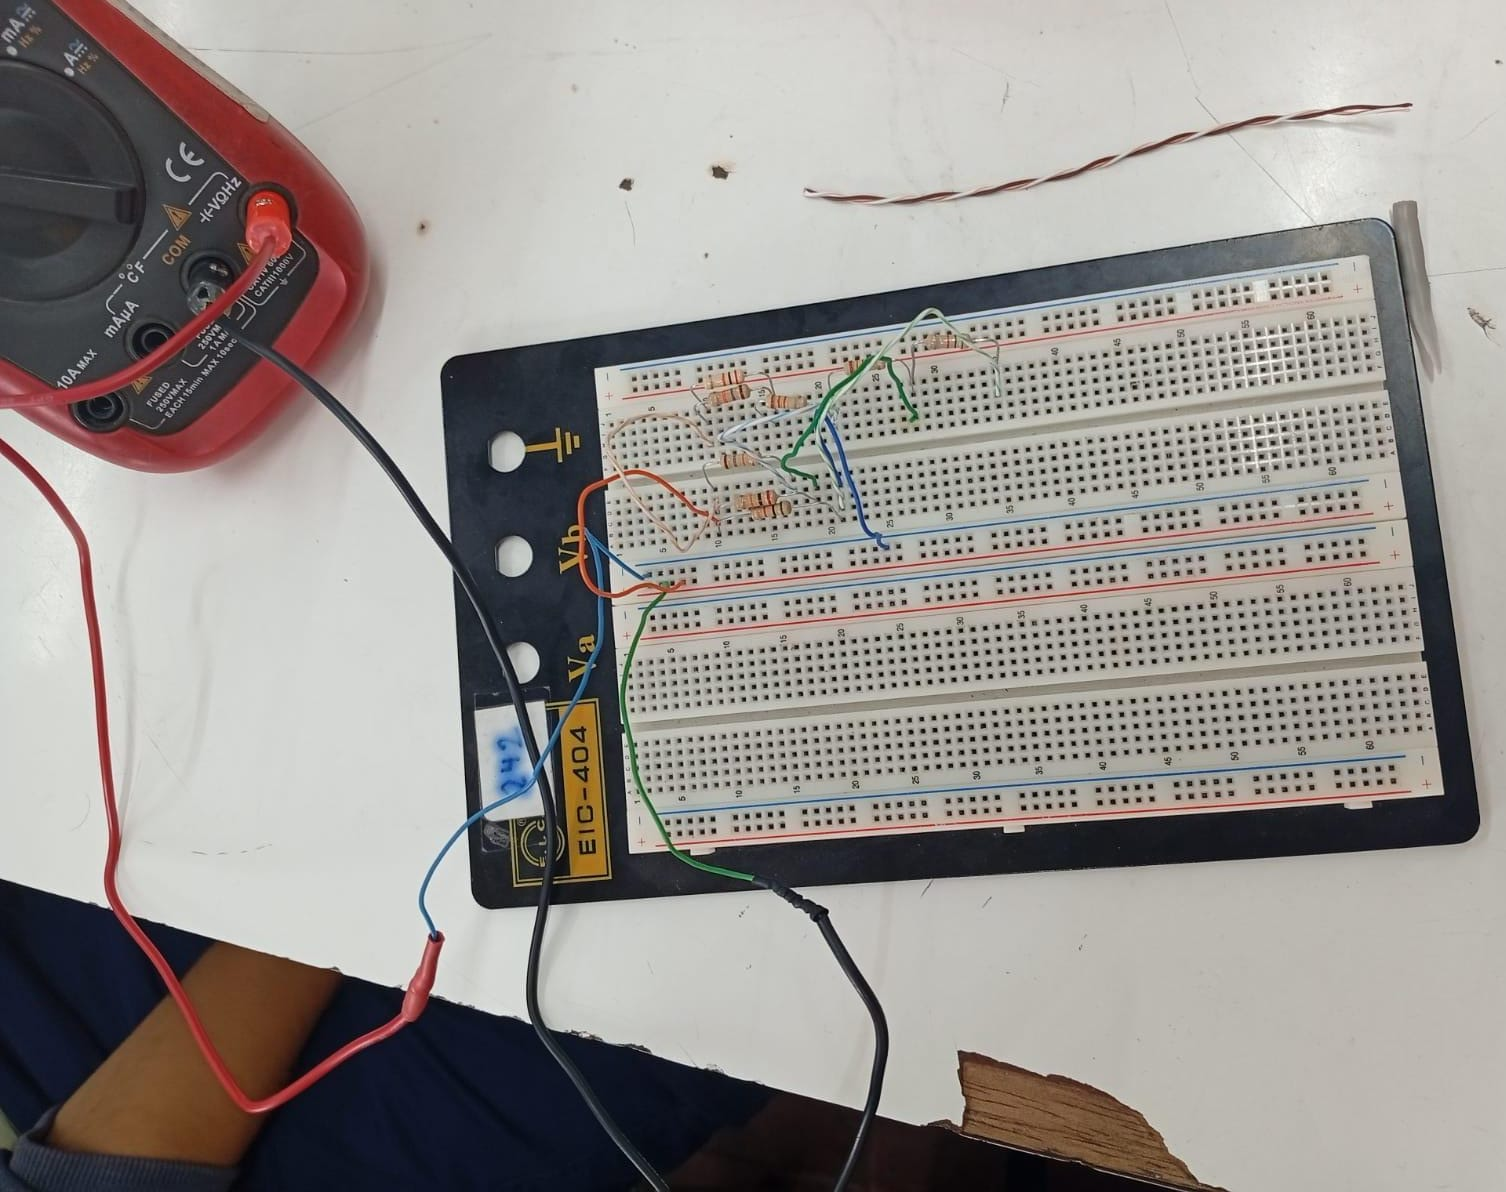
\includegraphics[width=\linewidth]{Imagen16.jpeg}
            \caption{Implementación práctica de la red resistiva}
            \label{ImplementacionRedResistiva}
        \end{minipage}
    \end{figure}
\end{enumerate}

\newpage
\subsection{PASO 2: Divisor de voltaje}
\begin{enumerate}
    \item Se armó el circuito del divisor de voltaje mostrado en la Figura \ref{CircuitoDivisorVoltaje} con $R_1=10\,\mathrm{k}\Omega$ y $R_2=10\,\mathrm{k}\Omega$ en el protoboard, pues estas eran las resistencias indicadas para que se cumpla que $V_{BC} / V_{AB} = 1/2$. Se midió el voltaje $V_{BC}$ y se comparó con el valor teórico obtenido con la ecuación \ref{eq:divisor-voltaje}. Se calculó el error relativo entre ambos valores. Los datos fueron anotados en las tablas \ref{tab:divisor-voltaje-r2} y \ref{tab:divisor-voltaje-vbc-1}.
    \begin{figure}[H]
        \centering
        \begin{minipage}{0.45\linewidth}
            \centering
            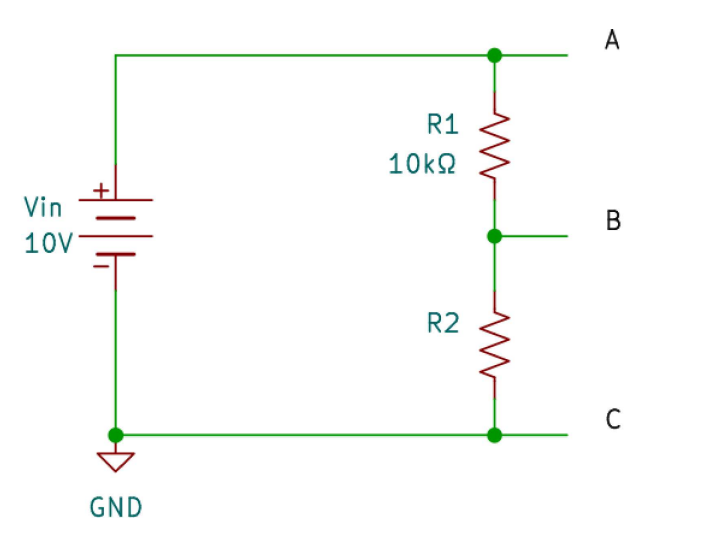
\includegraphics[width=\linewidth]{Imagen7.PNG}
            \caption{Circuito divisor de voltaje para $R_1=10\,\mathrm{k}\Omega$ y $R_2=10\,\mathrm{k}\Omega$}
            \label{CircuitoDivisorVoltaje}
        \end{minipage}
        \hspace{0.02\linewidth}
        \begin{minipage}{0.45\linewidth}
            \centering
            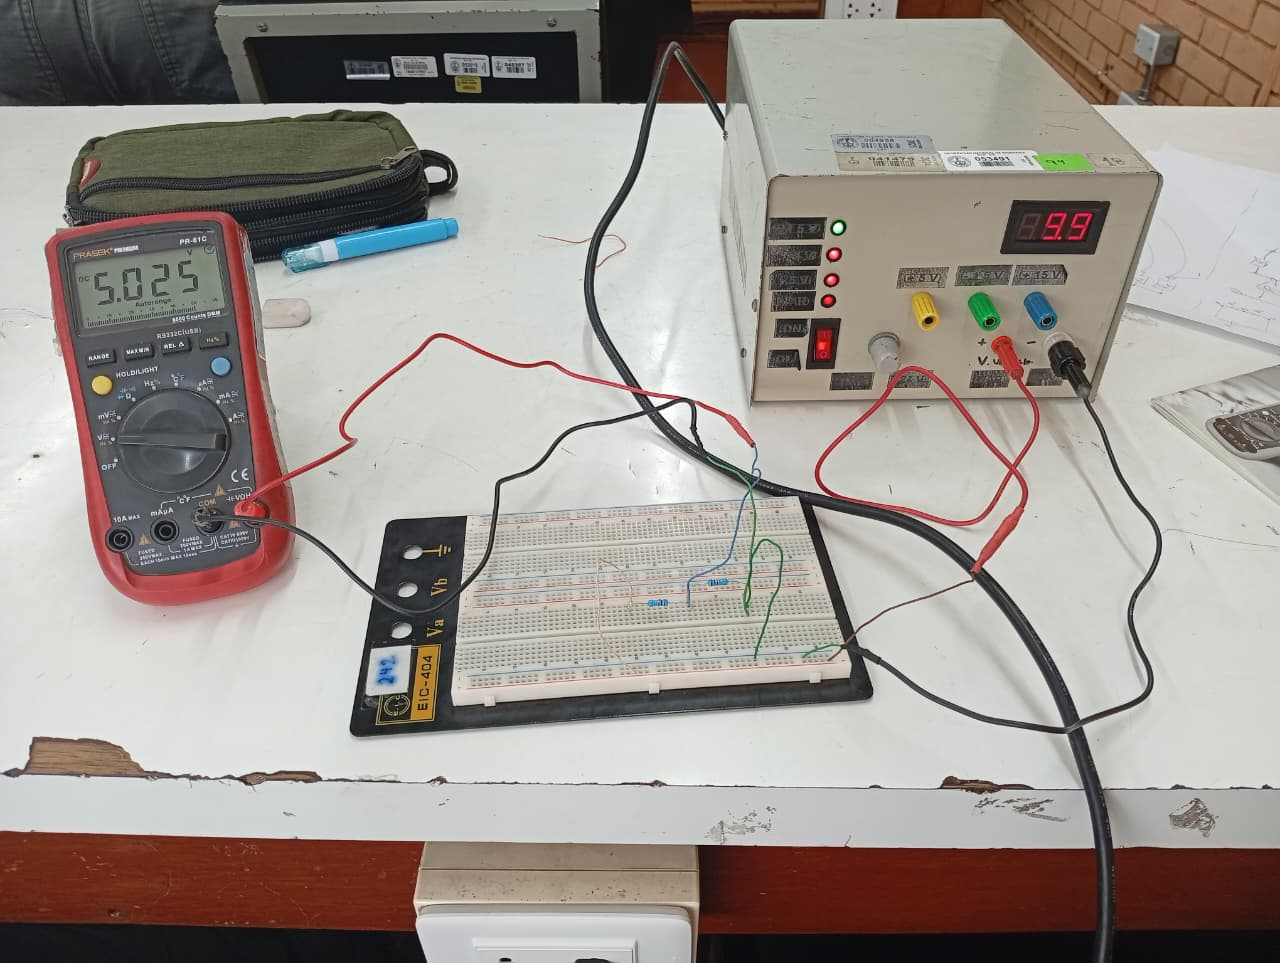
\includegraphics[width=\linewidth]{Imagen15.jpeg}
            \caption{Montaje experimental del divisor de voltaje}
            \label{MontajeDivisorVoltaje}
        \end{minipage}
    \end{figure}
    \bigskip
    \item Se colocó una resistencia $R_3$ en paralelo con $R_2$, tal que el valor de $R_3$ permitió que $V_{BC} / V_{AB} = 1/4$, este valor fue calculado teóricamente con la ecuación \ref{eq:divisor-voltaje-general}. Se midió el voltaje $V_{BC}$ y se comparó con el valor teórico obtenido con la ecuación \ref{eq:divisor-voltaje-general}. Se calculó el error relativo entre ambos valores. Los datos fueron anotados en las tablas \ref{tab:divisor-voltaje-r3} y \ref{tab:divisor-voltaje-vbc-2}.
    \item Se tomó un potenciómetro de $10k\Omega$ y otro de $100k\Omega$ y se puso en el circuito en lugar de $R_2$, de modo que al mover la perilla se obtengan diferentes resistencias y con ello varíe el valor de $V_{BC}$. Se midió el voltaje $V_{BC}$ para diferentes posiciones de la perilla y se comparó con los valores teóricos obtenidos con la ecuación \ref{eq:divisor-voltaje-general}. Se calculó el error relativo entre ambos valores. Los datos fueron anotados en las tablas \ref{tab:divisor-voltaje-potenciometro10k} y \ref{tab:divisor-voltaje-potenciometro100k}.
    \begin{figure}[H]
        \centering
        \begin{minipage}{0.45\linewidth}
            \centering
            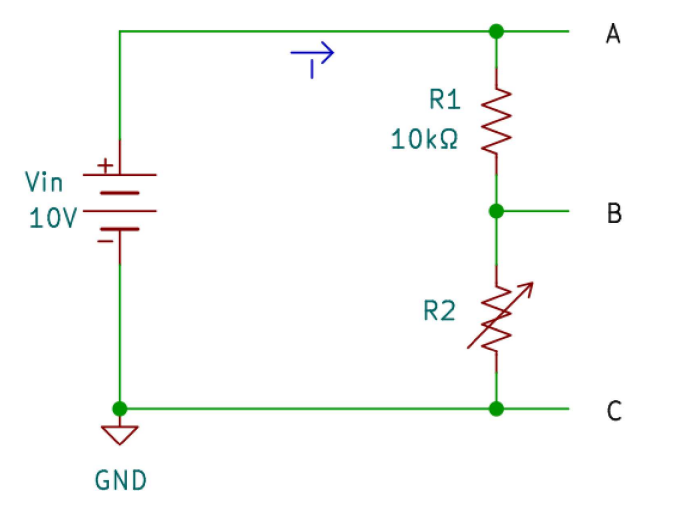
\includegraphics[width=\linewidth]{Imagen8.PNG}
            \caption{Circuito divisor de voltaje con potenciómetro de $10k\Omega$}
            \label{CircuitoDivisorVoltajePotenciometro}
        \end{minipage}
        \hspace{0.02\linewidth}
        \begin{minipage}{0.45\linewidth}
            \centering
            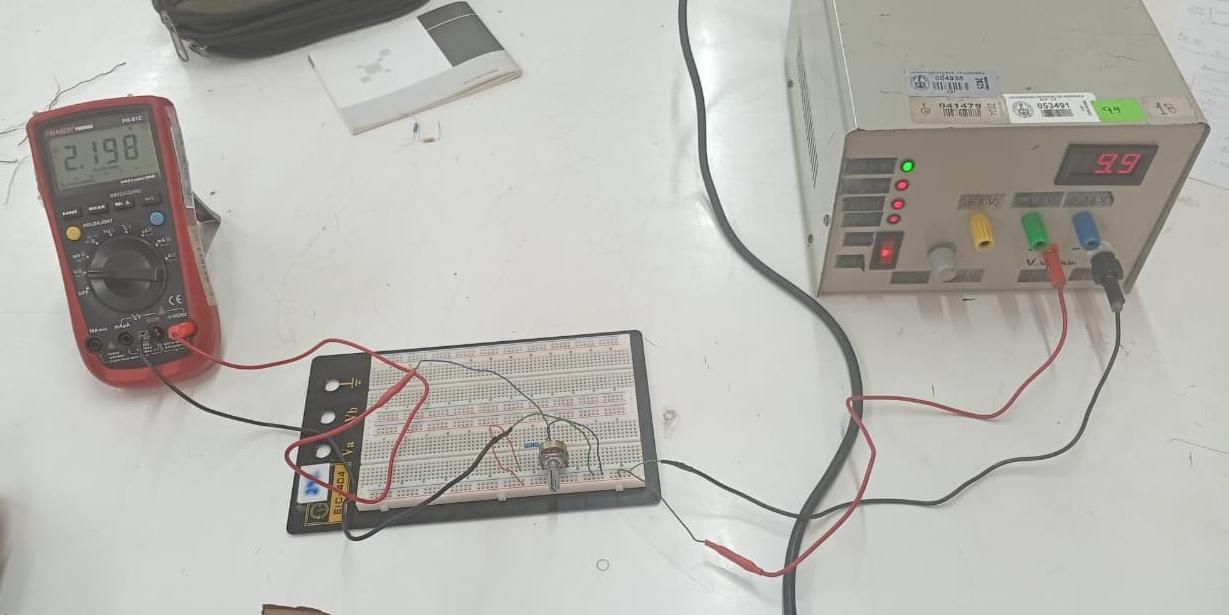
\includegraphics[width=\linewidth]{Imagen17.jpeg}
            \caption{Montaje experimental con potenciómetro}
            \label{MontajePotenciometro}
        \end{minipage}
    \end{figure}
\end{enumerate}

\bigskip
\subsection{PASO 3: Divisor de corriente}
\begin{enumerate}
    \item Se armó el circuito del divisor de corriente mostrado en la Figura \ref{CircuitoDivisorCorriente} con $R_1=10\,\mathrm{k}\Omega$ y $R_2=10\,\mathrm{k}\Omega$ en el protoboard, pues estas eran las resistencias indicadas para que se cumpla que $I_2 / I = 1/2$. Se midió la corriente $I_2$ y se comparó con el valor teórico obtenido con la ecuación \ref{eq:divisor-corriente}. Se calculó el error relativo entre ambos valores. Los datos fueron anotados en las tablas \ref{tab:divisor-corriente-r2} y \ref{tab:divisor-corriente-ir2-1}.
    \begin{figure}[H]
        \centering
        \begin{minipage}{0.45\linewidth}
            \centering
            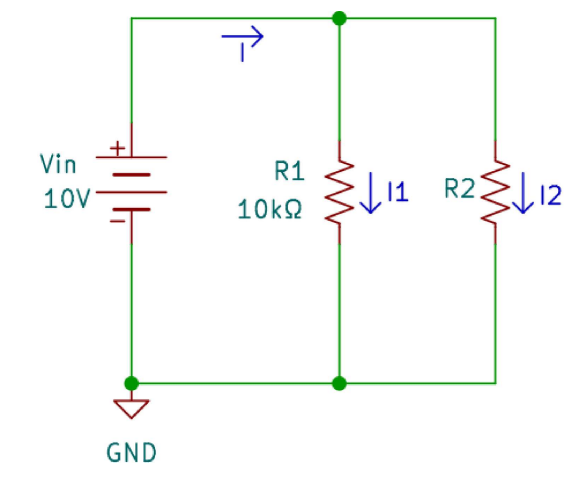
\includegraphics[width=\linewidth]{Imagen9.PNG}
            \caption{Circuito divisor de corriente para $R_1=10\,\mathrm{k}\Omega$ y $R_2=10\,\mathrm{k}\Omega$}
            \label{CircuitoDivisorCorriente}
        \end{minipage}
        \hspace{0.02\linewidth}
        \begin{minipage}{0.45\linewidth}
            \centering
            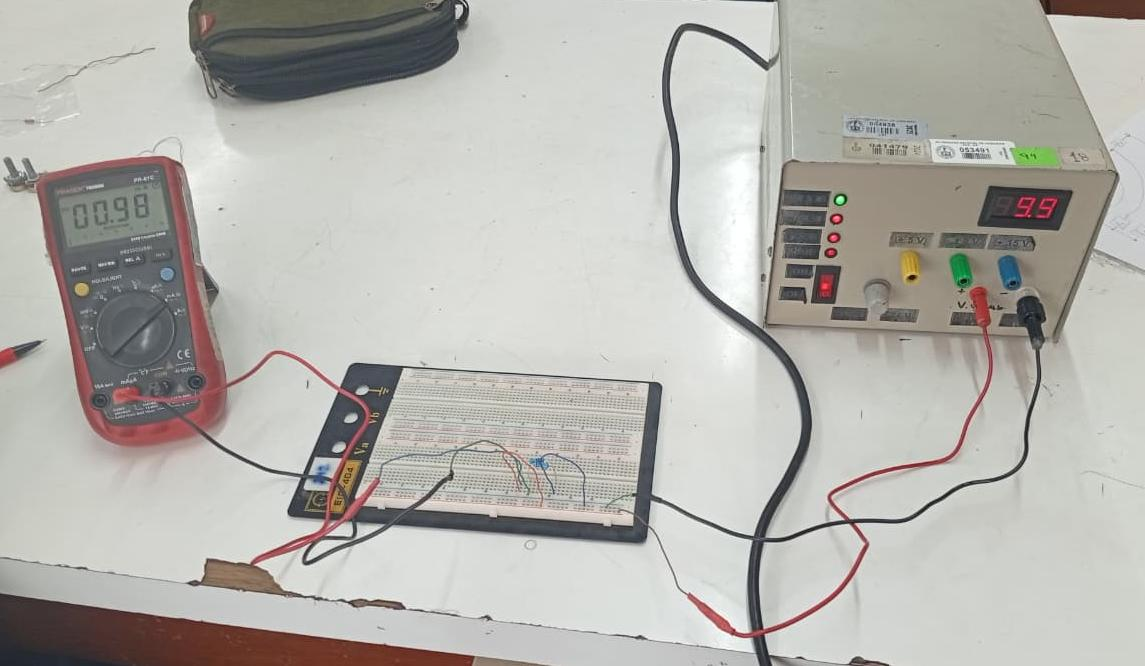
\includegraphics[width=\linewidth]{Imagen18.jpeg}
            \caption{Montaje experimental del divisor de corriente}
            \label{MontajeDivisorCorriente}
        \end{minipage}
    \end{figure}
    \item Se colocó una resistencia $R_3$ en paralelo con $R_2$, tal que el valor de $R_3$ permitió que $I_2 / I = 1/4$, este valor fue calculado teóricamente con la ecuación \ref{eq:divisor-corriente-general}. Se midió la corriente $I_2$ y se comparó con el valor teórico obtenido con la ecuación \ref{eq:divisor-corriente-general}. Se calculó el error relativo entre ambos valores. Los datos fueron anotados en las tablas \ref{tab:divisor-corriente-r3} y \ref{tab:divisor-corriente-ir2-2}.
\end{enumerate}

\tituloSeccion{Análisis de datos}
\subsection{Medición de resistencias}

\begin{table}[H]
    \centering
    \fontsize{10pt}{12pt}\selectfont
    \renewcommand{\arraystretch}{1.2}
    \setlength{\tabcolsep}{6pt}
    {
    \begin{tabular}{|C{5.1cm}|C{3.2cm}|C{3.3cm}|C{2.5cm}|}
    \hline
    \textbf{Colores de las franjas en el resistor} &
    \textbf{$R\,(\Omega)$ código de colores} &
    \textbf{Tolerancia ($\pm$) código de colores} &
    \textbf{$R\,(\Omega)$ Multímetro} \\
    \hline
    ROJO - MORADO - NEGRO - DORADO - MARRÓN & $270 \cdot 10^{-1} = 27,0$ & $\pm 1\%$ & $27,8$ \\
    \hline
    MARRÓN - GRIS - NEGRO - ROJO - MARRÓN & $180 \cdot 10^{2} = 18,0 \cdot 10^{3}$ & $\pm 2\%$ & $18,17 \cdot 10^{3}$ \\
    \hline
    ROJO - MORADO - MARRÓN - DORADO & $27 \cdot 10 = 270,0$ & $\pm 5\%$ & $265,6$ \\
    \hline
    MARRÓN - NEGRO - NEGRO - DORADO & $10 \cdot 1 = 10,0$ & $\pm 5\%$ & $10,6$ \\
    \hline
    AZUL - GRIS - NEGRO - DORADO & $68 \cdot 1 = 68,0$ & $\pm 5\%$ & $67,0$ \\
    \hline
    \end{tabular}}
\caption{Medición de resistencias por código de colores y multímetro.}
\label{tab:medicion-resistencias}
\end{table}

\textbf{ANÁLISIS:} Revisando de manera independiente cada resistencia, nos damos cuenta que el valor real de la primera no entra dentro de la tolerancia esperada. Sin embargo, el resto si cumple con este requisito.
\bigskip

\begin{table}[H]
    \centering
    \fontsize{10pt}{12pt}\selectfont
    \renewcommand{\arraystretch}{1.2}
    \setlength{\tabcolsep}{6pt}
    {
    \begin{tabular}{|C{1.45cm}|C{1.45cm}|C{1.45cm}|C{1.45cm}|C{1.45cm}|C{1.45cm}|C{1.45cm}|C{1.45cm}|}
    \hline
    \textbf{$R_1$ ($\Omega$)} &
    \textbf{$R_2$ ($\Omega$)} &
    \textbf{$R_3$ ($\Omega$)} &
    \textbf{$R_4$ ($\Omega$)} &
    \textbf{$R_5$ ($\Omega$)} &
    \textbf{$R_6$ ($\Omega$)} &
    \textbf{$R_7$ ($\Omega$)} &
    \textbf{$R_8$ ($\Omega$)} \\
    \hline
    $32,45\,\cdot\,10^{3}$ & $32,46\,\cdot\,10^{3}$ & $17,72\,\cdot\,10^{3}$ & $17,54\,\cdot\,10^{3}$ & $19,60\,\cdot\,10^{3}$ & $19,87\,\cdot\,10^{3}$ & $49,69\,\cdot\,10^{3}$ & $49,13\,\cdot\,10^{3}$ \\
    \hline
    \end{tabular}}
\caption{Valores medidos de las resistencias de la red mostrada en la figura 1.6.}
\label{tab:red-resistiva-resistencias}
\end{table}

\begin{table}[H]
    \centering
    \fontsize{10pt}{12pt}\selectfont
    \renewcommand{\arraystretch}{1.2}
    \setlength{\tabcolsep}{6pt}
    {
    \begin{tabular}{|C{4.0cm}|C{4.0cm}|C{4.0cm}|}
    \hline
    \textbf{$R_{eq}$ ($\Omega$) Calculado} &
    \textbf{$R_{eq}$ ($\Omega$) Medido} &
    \textbf{$\%$ error relativo} \\
    \hline
    $27,667\,\cdot\,10^{3}$ & $27,67\,\cdot\,10^{3}$ & $0,01$ \\
    \hline
    \end{tabular}}
\caption{Resistencia equivalente calculada, resistencia equivalente medida y error relativo.}
\label{tab:red-resistiva-resultados}
\end{table}

\textbf{ANÁLISIS:} El error relativo extremadamente bajo (0,01\%) entre el valor teórico calculado y el valor medido de la resistencia equivalente demuestra la precisión de la medición y la calidad del multímetro utilizado. Esta concordancia valida tanto los cálculos realizados como la correcta implementación del circuito en el protoboard.

\bigskip
\subsection{Divisor de voltaje}

\begin{table}[H]
    \centering
    \fontsize{10pt}{12pt}\selectfont
    \renewcommand{\arraystretch}{1.2}
    \setlength{\tabcolsep}{6pt}
    {
    \begin{tabular}{|C{3cm}|C{3cm}|C{3cm}|}
    \hline
    \textbf{Magnitud ($\Omega$) } & \textbf{Valor Teórico} & \textbf{Valor Real}\\
    \hline
    $R_2$ & $10\,\mathrm{k}\Omega$ & $9,98\,\mathrm{k}\Omega$ \\
    \hline
    \end{tabular}}
\caption{Selección de la resistencia $R_2$ para el divisor de voltaje.}
\label{tab:divisor-voltaje-r2}
\end{table}

\begin{table}[H]
    \centering
    \fontsize{10pt}{12pt}\selectfont
    \renewcommand{\arraystretch}{1.2}
    \setlength{\tabcolsep}{6pt}
    {
    \begin{tabular}{|C{4cm}|C{4cm}|C{4cm}|}
    \hline
    \textbf{$V_{BC}$ (V) Calculado} & \textbf{$V_{BC}$ (V) Medido} & \textbf{$\%$ error relativo} \\
    \hline
    $5$ & $5{,}025$ & $0{,}5\%$ \\
    \hline
    \end{tabular}}
\caption{Cálculo y medición de $V_{BC}$ para el primer montaje del divisor de voltaje.}
\label{tab:divisor-voltaje-vbc-1}
\end{table}

\textbf{ANÁLISIS:} El divisor de voltaje con resistencias iguales muestra un comportamiento muy próximo al teórico, con un error relativo de solo 0,5\%. La pequeña diferencia se debe principalmente a las tolerancias de las resistencias reales ($R_2 = 9,98\,\mathrm{k}\Omega$ en lugar de $10\,\mathrm{k}\Omega$ teórico) y posibles efectos de la impedancia interna del multímetro, confirmando la validez de la ecuación del divisor de voltaje.
\bigskip

\begin{table}[H]
    \centering
    \fontsize{10pt}{12pt}\selectfont
    \renewcommand{\arraystretch}{1.2}
    \setlength{\tabcolsep}{6pt}
    {
    \begin{tabular}{|C{3cm}|C{3cm}|C{3cm}|}
    \hline
    \textbf{Magnitud ($\Omega$)} & \textbf{Valor Teórico} & \textbf{Valor Real}\\
    \hline
    $R_3$ & $5\,\mathrm{k}\Omega$ & $4{,}99\,\mathrm{k}\Omega$ \\
    \hline
    \end{tabular}}
\caption{Selección de la resistencia $R_3$ para el segundo montaje del divisor de voltaje.}
\label{tab:divisor-voltaje-r3}
\end{table}

\begin{table}[H]
    \centering
    \fontsize{10pt}{12pt}\selectfont
    \renewcommand{\arraystretch}{1.2}
    \setlength{\tabcolsep}{6pt}
    {
    \begin{tabular}{|C{4cm}|C{4cm}|C{4cm}|}
    \hline
    \textbf{$V_{BC}$ (V) Calculado} & \textbf{$V_{BC}$ (V) Medido} & \textbf{$\%$ error relativo} \\
    \hline
    $2{,}5$ & $2{,}499$ & $0{,}04$ \\
    \hline
\end{tabular}}
\caption{Cálculo y medición de $V_{BC}$ para el segundo montaje del divisor de voltaje.}
\label{tab:divisor-voltaje-vbc-2}
\end{table}

\textbf{ANÁLISIS:} Al agregar $R_3$ en paralelo con $R_2$, se obtuvo una relación $V_{BC}/V_{AB} = 1/4$ con un error relativo de 0,04\%. Esta precisión confirma que el circuito se comporta exactamente como predice la teoría del divisor de voltaje modificado, y demuestra la efectividad de utilizar resistencias en paralelo para ajustar la proporción de voltaje deseada.

\bigskip
\begin{table}[H]
    \centering
    \fontsize{10pt}{12pt}\selectfont
    \renewcommand{\arraystretch}{1.2}
    \setlength{\tabcolsep}{6pt}
    {
    \begin{tabular}{|C{1cm}|C{1.8cm}|C{1.8cm}|C{1.8cm}|C{2cm}|C{1.8cm}|C{2cm}|}
    \hline
    \textbf{$R_2$ (k$\Omega$)} &
    \textbf{$V_{BC}$ (V) Calculado} &
    \textbf{$V_{BC}$ (V) Medido} &
    \textbf{$\%$ error relativo $V_{BC}$} &
    \textbf{$I$ (A) Calculado} &
    \textbf{$I$ (A) Medido} &
    \textbf{$\%$ error relativo $I$} \\
    \hline
    $5,24$ & $3,37$ & $3,33$ & $1,19\%$ & $0,64\cdot10^{-3}$ & $0,65\cdot10^{-3}$ & $1,56\%$ \\
    \hline
    $8,21$ & $4,46$ & $4,48$ & $0,45\%$ & $0,54\cdot10^{-3}$ & $0,54\cdot10^{-3}$ & $0\%$ \\
    \hline
    $10,13$ & $4,98$ & $5,00$ & $0,40\%$ & $0,49\cdot10^{-3}$ & $0,49\cdot10^{-3}$ & $0\%$ \\
    \hline
    $12,57$ & $5,51$ & $5,51$ & $0\%$ & $0,44\cdot10^{-3}$ & $0,44\cdot10^{-3}$ & $0\%$ \\
    \hline
    $15,12$ & $5.96$ & $5.98$ & $0,34\%$ & $0,39\cdot10^{-3}$ & $0,39\cdot10^{-3}$ & $0\%$ \\
    \hline
    \end{tabular}}
\caption{Mediciones para distintos valores de $R_2$ en el divisor de voltaje.}
\label{tab:divisor-voltaje-potenciometro10k}
\end{table}

\textbf{ANÁLISIS:} El potenciómetro de $10\,\mathrm{k}\Omega$ demuestra un comportamiento excelente como divisor de voltaje variable, con errores en voltaje menores al 1,2\% y errores en corriente prácticamente nulos. Se observa que conforme aumenta $R_2$, el voltaje $V_{BC}$ se acerca al voltaje de entrada, mientras que la corriente disminuye proporcionalmente, confirmando las predicciones teóricas del divisor de voltaje.
\bigskip

\begin{table}[H]
    \centering
    \fontsize{10pt}{12pt}\selectfont
    \renewcommand{\arraystretch}{1.2}
    \setlength{\tabcolsep}{6pt}
    {
    \begin{tabular}{|C{1cm}|C{1.8cm}|C{1.8cm}|C{1.8cm}|C{2cm}|C{1.8cm}|C{2cm}|}
    \hline
    \textbf{$R_2$ (k$\Omega$)} &
    \textbf{$V_{BC}$ (V) Calculado} &
    \textbf{$V_{BC}$ (V) Medido} &
    \textbf{$\%$ error relativo $V_{BC}$} &
    \textbf{$I$ (A) Calculado} &
    \textbf{$I$ (A) Medido} &
    \textbf{$\%$ error relativo $I$} \\
    \hline
    $20,51$ & $6,58$ & $6,55$ & $0,46\%$ & $0,32\cdot10^{-3}$ & $0,32\cdot10^{-3}$ & $0\%$ \\
    \hline
    $30,75$ & $7,40$ & $7,58$ & $2,43\%$ & $0,24\cdot10^{-3}$ & $0,24\cdot10^{-3}$ & $0\%$ \\
    \hline
    $40,46$ & $7,86$ & $7,84$ & $0,25\%$ & $0,19\cdot10^{-3}$ & $0,20\cdot10^{-3}$ & $5,26\%$ \\
    \hline
    $50,00$ & $8,17$ & $8,15$ & $0,24\%$ & $0,16\cdot10^{-3}$ & $0,15\cdot10^{-3}$ & $6,25\%$ \\
    \hline
    $71,3$ & $8,59$ & $8,58$ & $0,12\%$ & $0,12\cdot10^{-3}$ & $0,11\cdot10^{-3}$ & $8,33\%$ \\
    \hline
    \end{tabular}}
\caption{Mediciones para distintos valores de $R_2$ en el divisor de voltaje.2}
\label{tab:divisor-voltaje-potenciometro100k}
\end{table}

\textbf{ANÁLISIS:} Con el potenciómetro de $100\,\mathrm{k}\Omega$ se observa que los errores en voltaje permanecen bajos (menores al 2,5\%), confirmando el comportamiento del divisor. Asimismo, los errores en corriente se mantienen bajos para corrientes muy pequeñas, lo que sugiere que el multímetro es capaz de medir con precisión en este rango.
\bigskip

\subsection{Divisor de corriente}

\begin{table}[H]
    \centering
    \fontsize{10pt}{12pt}\selectfont
    \renewcommand{\arraystretch}{1.2}
    \setlength{\tabcolsep}{6pt}
    {
    \begin{tabular}{|C{3cm}|C{3cm}|C{3cm}|}
    \hline
    \textbf{Magnitud ($\Omega$)} & \textbf{Valor Teórico} & \textbf{Valor Real} \\
    \hline
    $R_2$ & $10\,\mathrm{k}\Omega$ & $9{,}98\,\mathrm{k}\Omega$ \\
    \hline
    \end{tabular}}
\caption{Selección de la resistencia $R_2$ para el divisor de corriente.}
\label{tab:divisor-corriente-r2}
\end{table}

\begin{table}[!ht]
    \centering
    \fontsize{10pt}{12pt}\selectfont
    \renewcommand{\arraystretch}{1.2}
    \setlength{\tabcolsep}{6pt}
    {
    \begin{tabular}{|C{4cm}|C{4cm}|C{4cm}|}
    \hline
    \textbf{$I_2$ (A) Calculado} & \textbf{$I_2$ (A) Medido} & \textbf{$\%$ error relativo} \\
    \hline
    $1\cdot10^{-3}$ & $0{,}98\cdot10^{-3}$ & $2$ \\
    \hline
    \end{tabular}}
\caption{Cálculo y medición de la corriente $I_2$ para el primer montaje del divisor de corriente.}
\label{tab:divisor-corriente-ir2-1}
\end{table}

\textbf{ANÁLISIS:} El divisor de corriente con resistencias iguales presenta un error relativo de 2\%, ligeramente mayor que los obtenidos en el divisor de voltaje. Esta diferencia puede atribuirse a que las mediciones de corriente requieren insertar el amperímetro en serie con el circuito, lo que puede introducir pequeñas perturbaciones adicionales debido a la impedancia interna del multímetro, aunque el resultado sigue siendo satisfactorio y valida la ecuación del divisor de corriente.

\begin{table}[H]
    \centering
    \fontsize{10pt}{12pt}\selectfont
    \renewcommand{\arraystretch}{1.2}
    \setlength{\tabcolsep}{6pt}
    {
    \begin{tabular}{|C{3cm}|C{3cm}|C{3cm}|}
    \hline
    \textbf{Magnitud ($\Omega$)} & \textbf{Valor Teórico} & \textbf{Valor Real} \\
    \hline
    $R_3$ & $20\,\mathrm{k}\Omega$ & $19{,}98\,\mathrm{k}\Omega$ \\
    \hline
    \end{tabular}}
\caption{Selección de la resistencia $R_3$ para el segundo montaje del divisor de corriente.}
\label{tab:divisor-corriente-r3}
\end{table}

\begin{table}[H]
    \centering
    \fontsize{10pt}{12pt}\selectfont
    \renewcommand{\arraystretch}{1.2}
    \setlength{\tabcolsep}{6pt}
    {
    \begin{tabular}{|C{4cm}|C{4cm}|C{4cm}|}
    \hline
    \textbf{$I_2$ (A) Calculado} & \textbf{$I_2$ (A) Medido} & \textbf{$\%$ error relativo} \\
    \hline
    $0{,}33\cdot10^{-3}$ & $0{,}33\cdot10^{-3}$ & $0$ \\
    \hline
    \end{tabular}}
\caption{Cálculo y medición de la corriente $I_2$ para el segundo montaje del divisor de corriente.}
\label{tab:divisor-corriente-ir2-2}
\end{table}

\textbf{ANÁLISIS:} El segundo montaje del divisor de corriente, con $R_3$ en paralelo que logra la relación $I_2/I = 1/4$, muestra una concordancia perfecta (error relativo del 0\%) entre el valor teórico y el medido. Este resultado excepcional confirma la precisión del cálculo de la resistencia equivalente en paralelo y valida completamente la ecuación generalizada del divisor de corriente para circuitos con múltiples resistencias.
\bigskip

\newpage
\tituloSeccion{Discusión de resultados}
Los resultados obtenidos demuestran una excelente concordancia entre los valores teóricos y experimentales, validando tanto los modelos teóricos como la calidad de la instrumentación utilizada.

\subsection{Análisis de la medición de resistencias}
En la medición individual de resistencias, se observó que 4 de las 5 resistencias evaluadas cumplieron con las tolerancias especificadas por el código de colores, representando un 80\% de confiabilidad. La resistencia de 27 $\Omega$ mostró una desviación del 2,96\% respecto al valor nominal, excediendo su tolerancia del ±1\%. Esta discrepancia puede atribuirse a factores como envejecimiento del componente o daños durante su uso previo.

El análisis de la red resistiva compleja mostró una precisión excepcional, incluso inesperada, con un error relativo de apenas 0,01\%, lo que demuestra que las leyes de combinación de resistencias (series y paralelos) se cumplen en condiciones prácticas.

\subsection{Comportamiento de los divisores de voltaje}
Los divisores de voltaje exhibieron un rendimiento muy bueno en todas las configuraciones probadas. El divisor básico con resistencias iguales (10 k$\Omega$ cada una) presentó un error de solo 0,5\%, mientras que la configuración modificada con $R_3$ en paralelo logró un error de 0,04\%, demostrando que la adición de resistencias en paralelo es una técnica efectiva para ajustar con precisión las relaciones de voltaje.

Los experimentos con potenciómetros revelaron comportamientos interesantes: el potenciómetro de 10 k$\Omega$ mostró errores máximos de 1,19\% en voltaje, mientras que el de 100 k$\Omega$ presentó errores de hasta 2,43\%. Consideramos que esta diferencia se debe principalmente a la fácil variación de resistencia en el potenciómetro al sacarlo del protoboard (donde se mide) y ponerlo otra vez en el circuito.

\subsection{Análisis de los divisores de corriente}
Los divisores de corriente mostraron errores ligeramente mayores que los de voltaje (2\% vs 0,5\%), lo cual es consistente con las características intrínsecas de ambos tipos de medición. Se sabe que las mediciones de corriente requieren la inserción del amperímetro en serie, introduciendo su impedancia interna al circuito, mientras que las mediciones de voltaje se realizan en paralelo con impedancia muy alta, minimizando la perturbación del circuito original.

La configuración modificada del divisor de corriente alcanzó una precisión perfecta (error 0\%), sugiriendo que para ciertas combinaciones de valores de resistencia, los efectos de la impedancia interna del multímetro se compensan naturalmente.

\subsection{Efectos de la impedancia del multímetro}
El análisis de los datos revela que la impedancia del multímetro (3000 M$\Omega$ en escalas bajas y 10 M$\Omega$ en escalas altas) tiene un impacto prácticamente despreciable en las mediciones de voltaje, como se evidencia en los errores consistentemente bajos. Sin embargo, en las mediciones de corriente, especialmente en el rango de microamperios (como en el potenciómetro de 100 k$\Omega$), se observan variaciones mayores que pueden atribuirse a las limitaciones de resolución del instrumento en escalas muy sensibles.

\tituloSeccion{Actividades adicionales}
\begin{itemize}
    \item Muestre cómo obtuvo teóricamente el resistor equivalente en el circuito de la Figura \ref{CircuitoRedResistiva}
    \item Usando los datos del paso 2, ¿se podrá obtener el valor de la impedancia del multímetro cuando este se usa para medir voltaje? Justifique su respuesta.
    \item Diseñe un experimento que permita determinar la resistencia interna del multímetro cuando se mide corriente eléctrica. Elabore un diagrama del circuito, explique el procedimiento y justifique los cálculos necesarios.
\end{itemize}

\subsection{Cálculo teórico del resistor equivalente}

Para obtener el resistor equivalente del circuito de la Figura \ref{CircuitoRedResistiva}, se debe analizar la configuración de las resistencias entre los puntos A y B siguiendo la secuencia de conexiones del circuito.

\textbf{Paso 1:} $R_4$ y $R_6$ están en paralelo
\begin{equation}
R_{46} = \frac{R_4 \cdot R_6}{R_4 + R_6} = \frac{17,54 \times 19,87}{17,54 + 19,87} = \frac{348,54}{37,41} = 9,32 \, \mathrm{k}\Omega
\end{equation}

\textbf{Paso 2:} $R_{46}$ está en serie con $R_1$
\begin{equation}
R_{146} = R_1 + R_{46} = 32,45 + 9,32 = 41,77 \, \mathrm{k}\Omega
\end{equation}

\textbf{Paso 3:} $R_{146}$ está en paralelo con $R_3$
\begin{equation}
R_{1346} = \frac{R_{146} \cdot R_3}{R_{146} + R_3} = \frac{41,77 \times 17,72}{41,77 + 17,72} = \frac{740,57}{59,49} = 12,45 \, \mathrm{k}\Omega
\end{equation}

\textbf{Paso 4:} $R_{1346}$ está en serie con $R_2$
\begin{equation}
R_{21346} = R_2 + R_{1346} = 32,46 + 12,45 = 44,91 \, \mathrm{k}\Omega
\end{equation}

\textbf{Paso 5:} $R_{21346}$ está en paralelo con $R_5$
\begin{equation}
R_{521346} = \frac{R_{21346} \cdot R_5}{R_{21346} + R_5} = \frac{44,91 \times 19,60}{44,91 + 19,60} = \frac{880,24}{64,51} = 13,65 \, \mathrm{k}\Omega
\end{equation}

\textbf{Paso 6:} $R_{521346}$ está en serie con $R_7$
\begin{equation}
R_{7521346} = R_7 + R_{521346} = 49,69 + 13,65 = 63,34 \, \mathrm{k}\Omega
\end{equation}

\textbf{Paso 7:} $R_{7521346}$ está en paralelo con $R_8$ (resistencia equivalente final)
\begin{equation}
R_{eq(A-B)} = \frac{R_{7521346} \cdot R_8}{R_{7521346} + R_8} = \frac{63,34 \times 49,13}{63,34 + 49,13} = \frac{3111,32}{112,47} = 27,67 \, \mathrm{k}\Omega
\end{equation}

\bigskip
\subsection{Determinación de la impedancia del multímetro}

Para determinar la impedancia interna del multímetro cuando se usa para medir voltaje, utilizaremos los datos del divisor de voltaje del paso 2.

\textbf{Análisis teórico:}
Cuando el multímetro se conecta en paralelo para medir voltaje, su impedancia interna $R_{mult}$ se coloca en paralelo con la rama donde se mide $V_{BC}$, de modo que el voltaje observado puede variar ligeramente respecto al valor ideal.

Para el divisor de voltaje básico con $R_1 = 10 \, \mathrm{k}\Omega$ y $R_2 = 10 \, \mathrm{k}\Omega$:
\begin{itemize}
    \item Sin multímetro: $V_{BCideal} = V_{in} \cdot \frac{R_2}{R_1 + R_2} = 10 \cdot \frac{10}{10 + 10} = 5{,}0 \, \mathrm{V}$
    \item Con multímetro: $V_{BCmedido} = 5{,}025 \, \mathrm{V}$
\end{itemize}

Si se modela el multímetro como una carga resistiva, la resistencia equivalente de la rama medida es:
\begin{equation}
R_{eq} = \frac{R_2 \cdot R_{mult}}{R_2 + R_{mult}}
\end{equation}

En un divisor de voltaje, esa resistencia equivalente puede despejarse a partir de la razón $x = V_{BC}/V_{in}$:
\begin{equation}
R_{eq} = \frac{x \, R_1}{1 - x}
\end{equation}

Usando los datos medidos:
\begin{equation}
x = \frac{5{,}025}{10} = 0{,}5025
\end{equation}

por lo tanto,
\begin{equation}
R_{eq} = \frac{0{,}5025 \cdot 10 \, \mathrm{k}\Omega}{1 - 0{,}5025} = 10{,}10 \, \mathrm{k}\Omega
\end{equation}

Sin embargo, en un paralelo entre dos resistencias positivas siempre debe cumplirse que $R_{eq} < R_2$. Como aquí se obtiene $R_{eq} \approx 10{,}10 \, \mathrm{k}\Omega > R_2 = 9{,}98 \, \mathrm{k}\Omega$, la ecuación
\begin{equation}
R_L = \frac{R_2 \cdot R_{mult}}{R_2 + R_{mult}}
\end{equation}
no admite una solución física con $R_{mult} > 0$. Si se despeja algebraicamente, aparece un valor negativo, pero eso no representa una impedancia real: únicamente indica que los datos no son consistentes con un efecto de carga medible del multímetro.

\textbf{Conclusión:}
Con los datos del paso 2 no es posible determinar la impedancia interna del multímetro. La lectura está dentro del orden de la incertidumbre experimental y, además, la impedancia de entrada típica del instrumento es muy alta (aproximadamente $10 \, \mathrm{M}\Omega$ en las escalas de voltaje), por lo que su efecto de carga sobre un divisor de resistencias de $10 \, \mathrm{k}\Omega$ es prácticamente despreciable.

\bigskip
\tituloSeccion{Conclusiones}

\subsection{Conclusiones sobre mediciones de resistencias}
\begin{itemize}
    \item Se logró realizar exitosamente mediciones eléctricas básicas en circuitos resistivos, validando el uso del multímetro digital modelo PRASEK PREMIUM PR-61C como instrumento de precisión para este tipo de experimentos, con errores relativos promedio inferiores al 1\%.
    \item La aplicación del código de colores para resistencias demostró ser confiable en el 80\% de los casos evaluados, con solo una resistencia (27 $\Omega$) fuera del rango de tolerancia especificado, lo que subraya la importancia de verificar los valores nominales con mediciones directas antes del uso.
    \item El análisis de la red resistiva compleja evidenció la precisión extraordinaria del cálculo teórico de resistencias equivalentes, con un error relativo de apenas 0,01\%.
\end{itemize}

\subsection{Conclusiones sobre divisores de voltaje}
\begin{itemize}
    \item Los circuitos divisores de voltaje mostraron un comportamiento altamente estable, con errores relativos menores al 2,5\% en todas las configuraciones probadas.
    \item La técnica de agregar resistencias en paralelo para modificar las relaciones de voltaje demostró ser efectiva, logrando una precisión de 0,04\% en la configuración $V_{BC}/V_{AB} = 1/4$.
    \item El uso de potenciómetros como resistencias variables confirmó la versatilidad de estos componentes para generar divisores de voltaje ajustables, manteniendo errores menores al 2,5\% en todo el rango de operación.
\end{itemize}

\subsection{Conclusiones sobre divisores de corriente}
\begin{itemize}
    \item Los divisores de corriente presentaron resultados satisfactorios con errores máximos del 2\%, ligeramente superiores a los divisores de voltaje debido a las perturbaciones introducidas por la medición en serie y la impedancia interna del multímetro, pero aún dentro de rangos aceptables para aplicaciones de laboratorio.
    \item La configuración modificada del divisor de corriente con $R_3$ en paralelo alcanzó una precisión perfecta (error 0\%), validando completamente la ecuación generalizada del divisor de corriente y demostrando que para ciertas combinaciones de resistencias, los efectos instrumentales se pueden minimizar significativamente.
\end{itemize}

\subsection{Conclusiones sobre la influencia del multímetro}
\begin{itemize}
    \item Se confirmó experimentalmente que la impedancia interna del multímetro (10 M$\Omega$ para escalas altas, 3000 M$\Omega$ para escalas bajas) influye de manera diferente según el tipo de medición: prácticamente despreciable en mediciones de voltaje debido a su alta impedancia, pero más significativa en mediciones de corriente, especialmente en rangos de microamperios.
    \end{itemize}

\tituloSeccion{Bibliografía}
    \begin{itemize}
        \item JAMES J. BROPHY, \textit{Basic electronics for scientists}, $5^{Th}$ Edition, McGraw Hill.
        \item UNI-FC, \textit{Circuitos Electrónicos Analógicos: Guía de laboratorio del experimento 1 y 2}, 2026
    \end{itemize}

\tituloSeccion{Anexos}

\begin{figure}[H]
    \centering
    \begin{minipage}{0.48\linewidth}
        \centering
        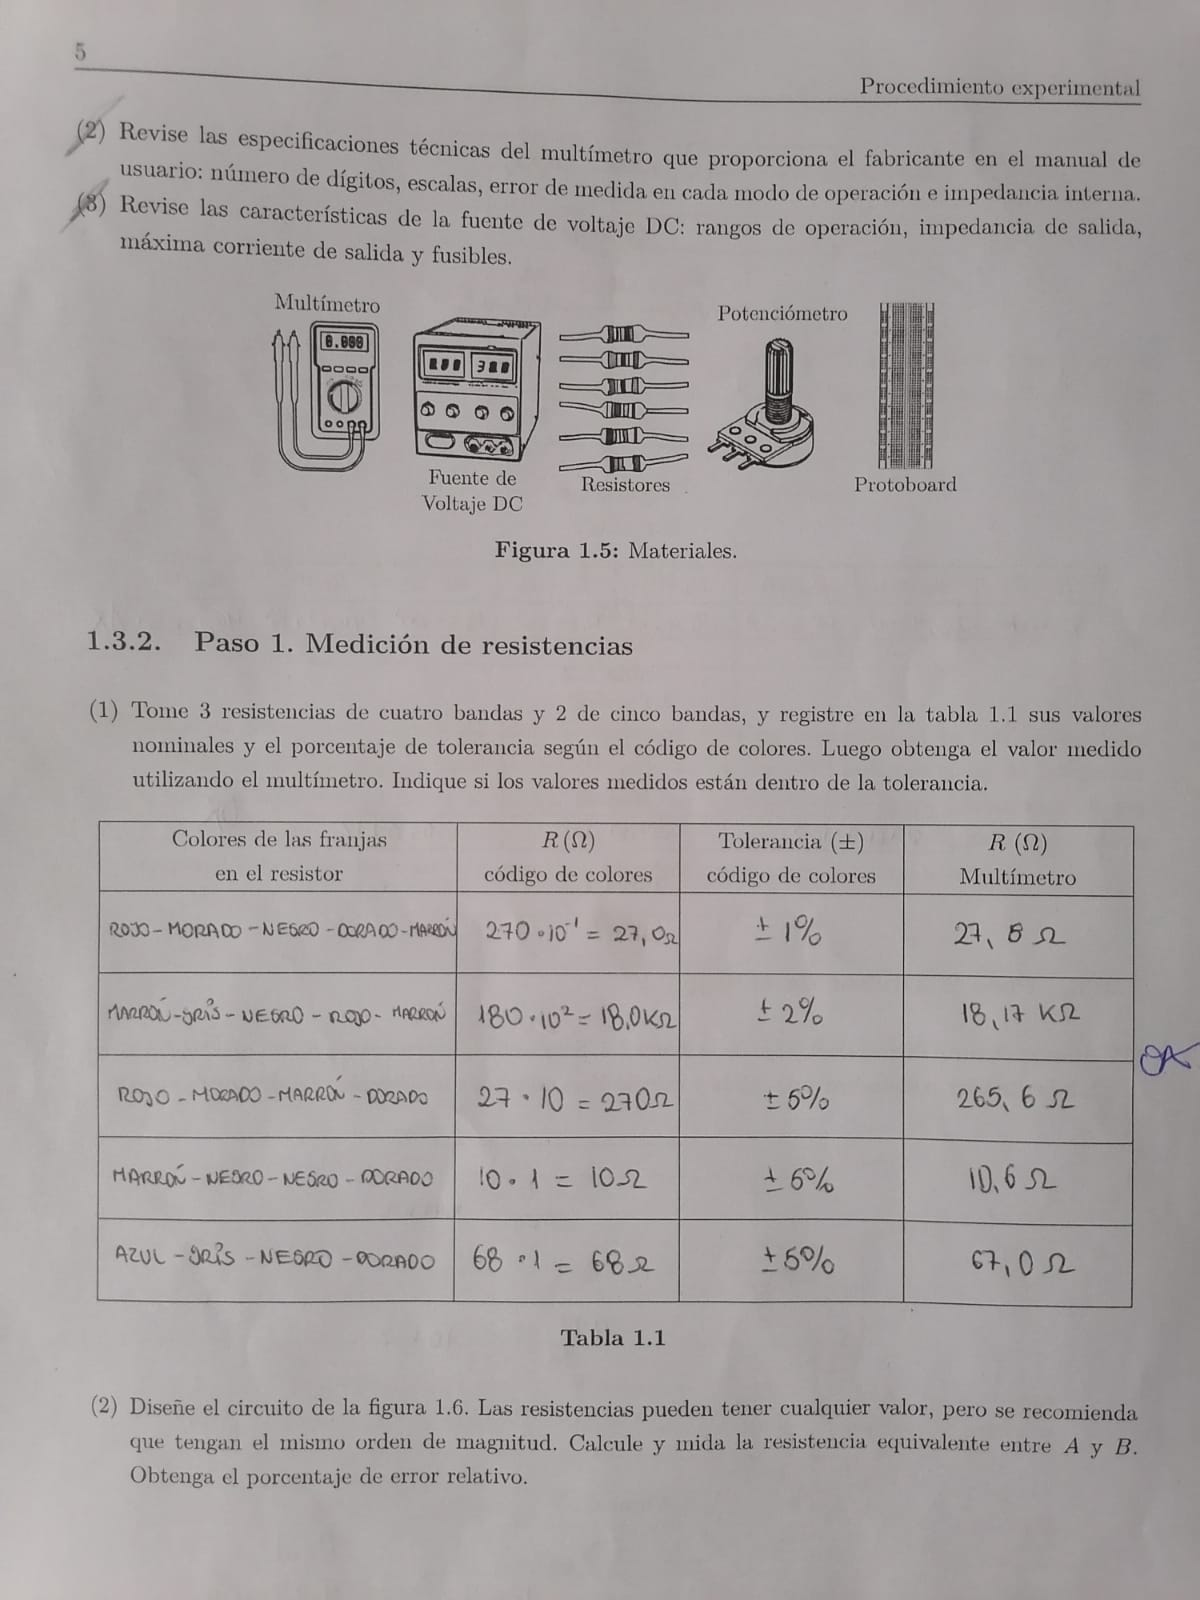
\includegraphics[width=\linewidth]{Imagen10.jpeg}
        \caption{Anexo 1: Configuración experimental adicional}
        \label{anexo1}
    \end{minipage}
    \hspace{0.02\linewidth}
    \begin{minipage}{0.48\linewidth}
        \centering
        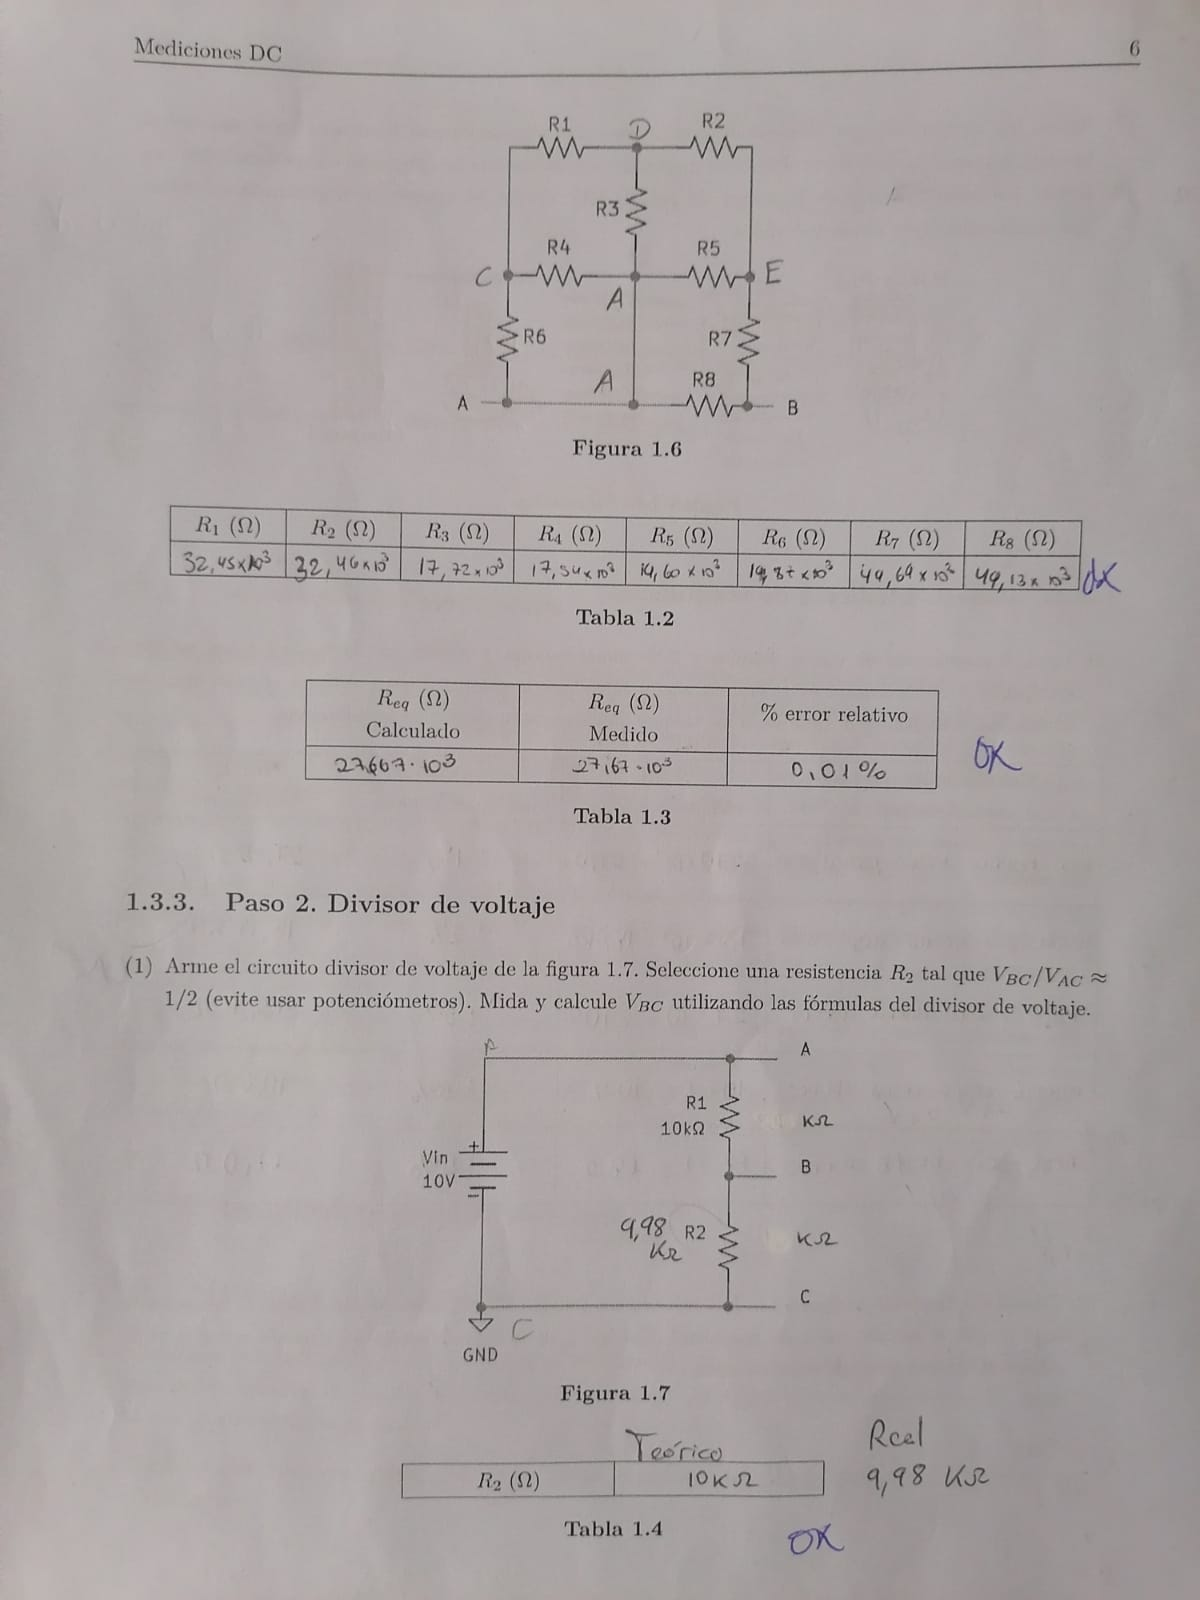
\includegraphics[width=\linewidth]{Imagen11.jpeg}
        \caption{Anexo 2: Mediciones complementarias}
        \label{anexo2}
    \end{minipage}
\end{figure}

\begin{figure}[H]
    \centering
    \begin{minipage}{0.48\linewidth}
        \centering
        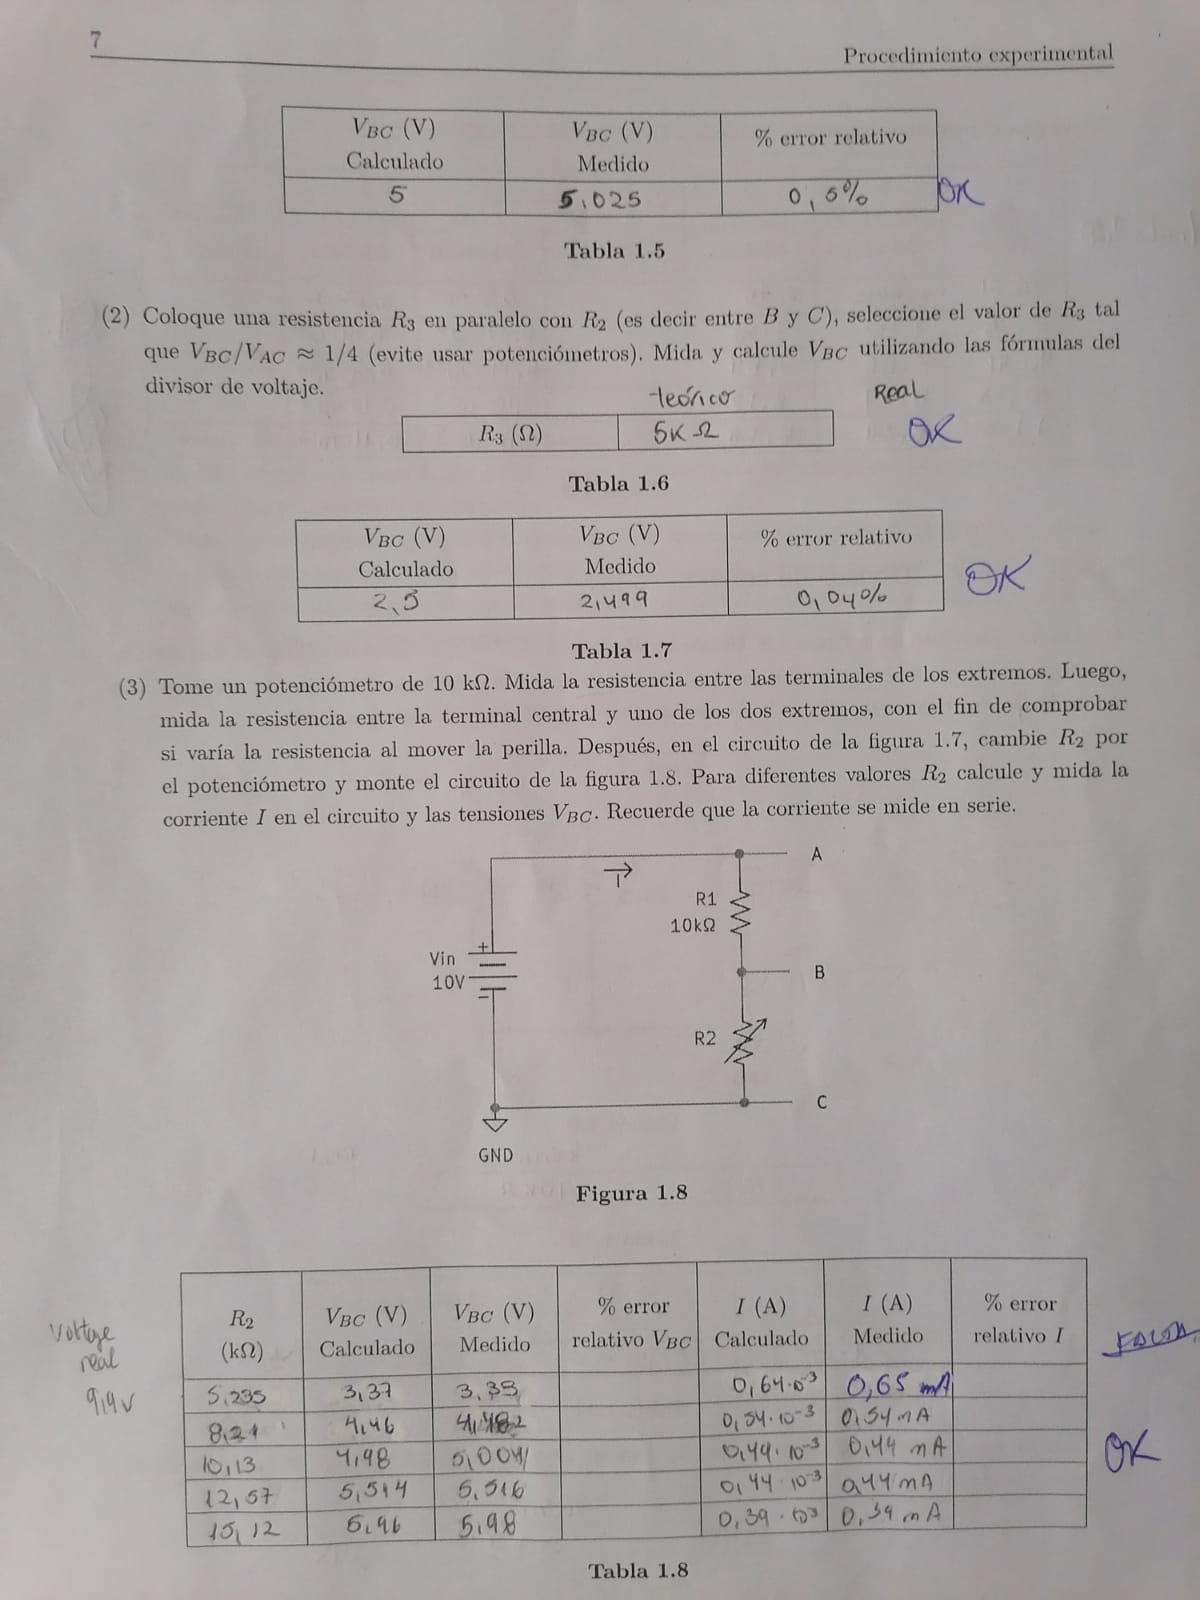
\includegraphics[width=\linewidth]{Imagen12.jpeg}
        \caption{Anexo 3: Análisis de circuitos adicionales}
        \label{anexo3}
    \end{minipage}
    \hspace{0.02\linewidth}
    \begin{minipage}{0.48\linewidth}
        \centering
        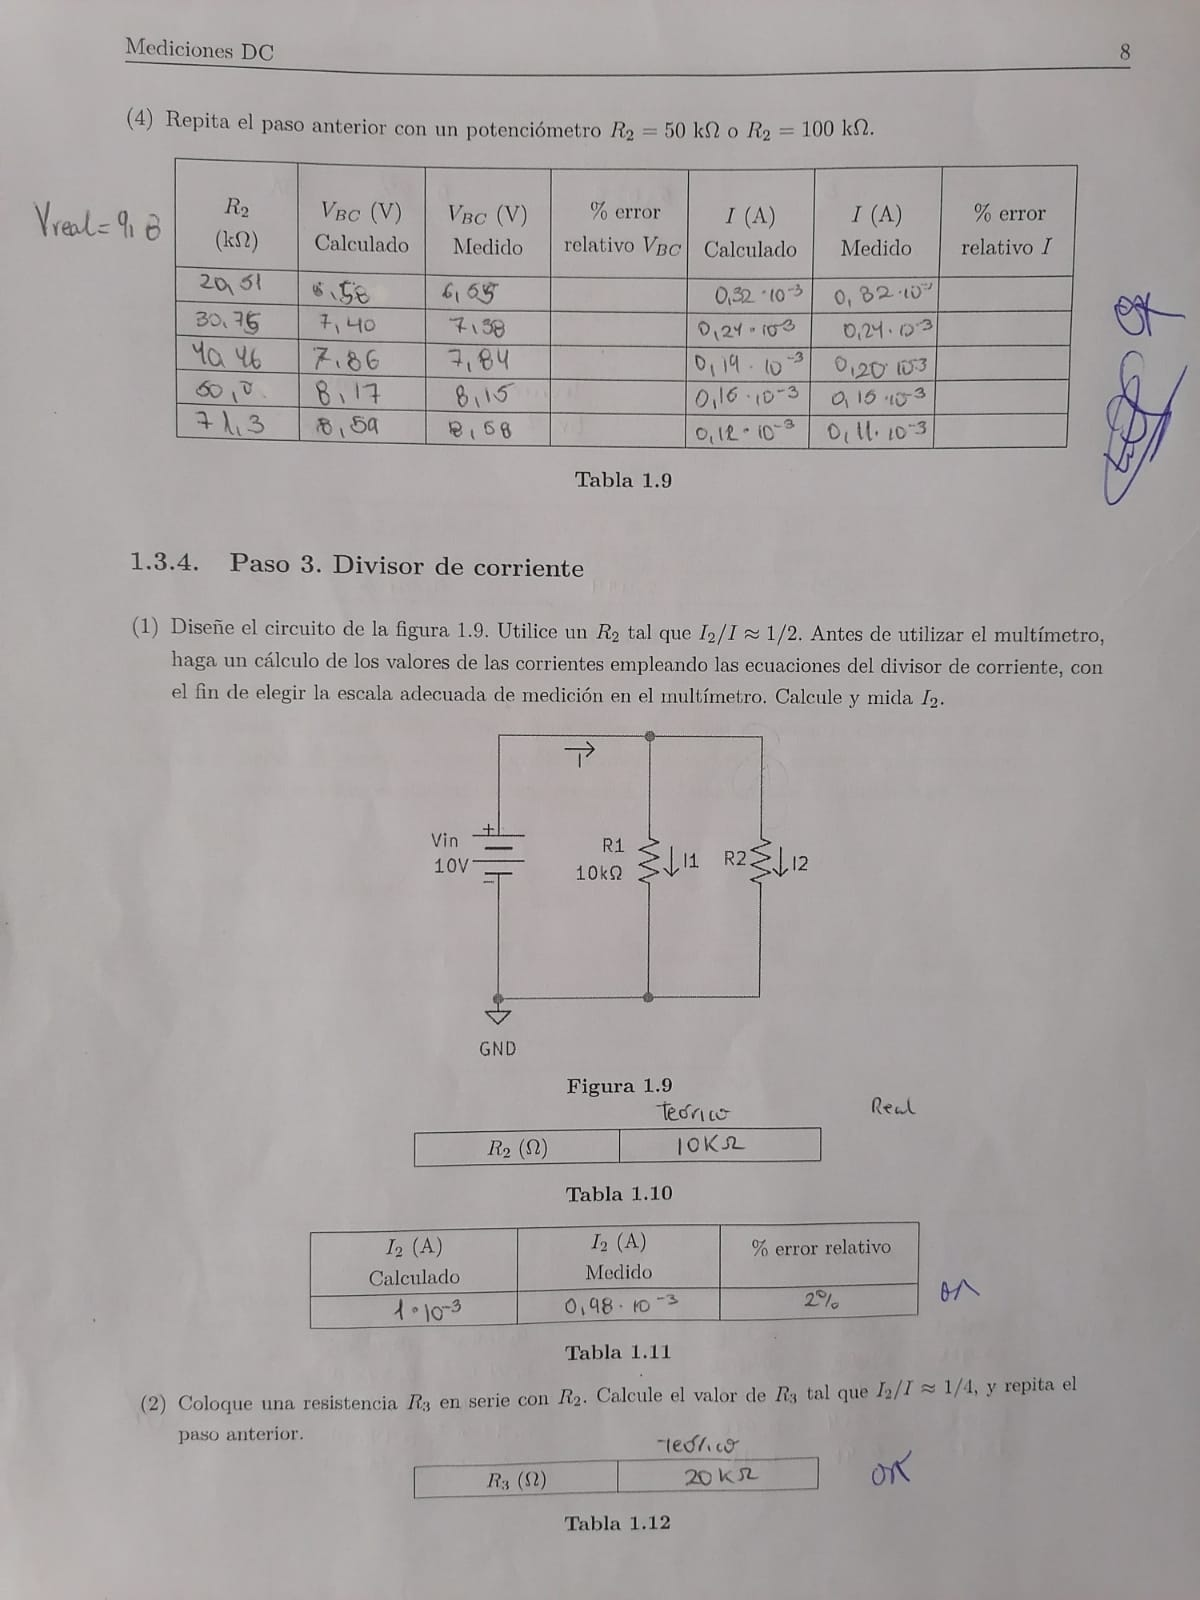
\includegraphics[width=\linewidth]{Imagen13.jpeg}
        \caption{Anexo 4: Verificación de resultados experimentales}
        \label{anexo4}
    \end{minipage}
\end{figure}

\begin{figure}[H]
    \centering
    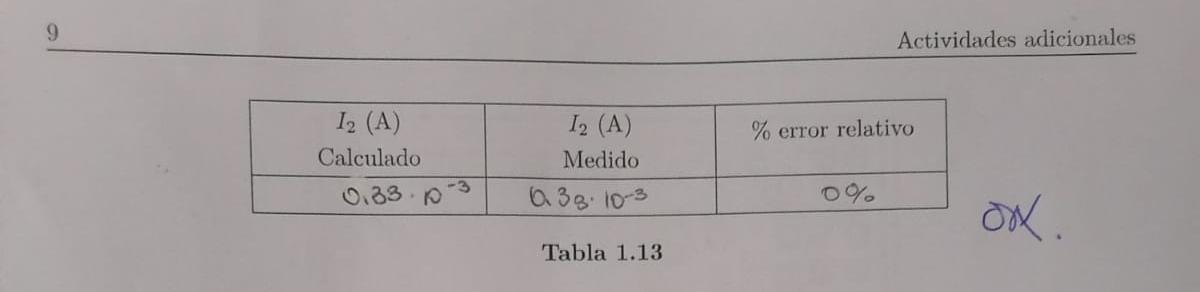
\includegraphics[width=0.6\linewidth]{Imagen14.jpeg}
    \caption{Anexo 5: Documentación adicional del experimento}
    \label{anexo5}
\end{figure}

\end{document}
